\documentclass[notes]{beamer}
\usetheme[numbering=fraction, progressbar=frametitle]{metropolis}
\setbeamercovered{transparent}

\usepackage[utf8]{inputenc}
\usepackage[T1]{fontenc}
\usepackage{lmodern}

\title{Zukunft der Raumfahrt}
\date{\today}
\author{Jens Juhl, Torben Mehner}
\institute{KIT}
\begin{document}
\maketitle

\begin{frame}{Inhaltsverzeichnis}
	\tableofcontents[sectionstyle=show,subsectionstyle=show]
\end{frame}

\section{Nahe Zukunft}
\subsection{NASA - Journey to Mars}
\begin{frame}{\insertsection: \insertsubsection}
	\begin{minipage}{.45\textwidth}
		Heute - Mitte 2020: \\
		\textbf{Earth Reliant} \\
		\note<1>{Earth Reliant
			\begin{itemize}
				\item ISS bis 2024
				\item Kommerzielle Raumfahrt im erdnahen Orbit
				\item Entwicklung von Systemen für interplanetare Raumfahrt
			\end{itemize}}
		
		\pause
		
		2018 - 2030: \\
		\textbf{Proving Ground} \\
		\note<2>{
			Proving Ground
			\begin{itemize}
				\item Regelmäßige, bemannte Missionen im Mondorbit
				\item Durch jahrelange Missionen beweisen, dass Habitate im 
				weiten All funktionieren
				\item Einfangen eines Asteroids und Platzierung im Mond-Orbit. 
				Dann sollen Astronuten robotergestützt Proben nehmen.
			\end{itemize}
			}
		\pause
		
		Heute - 2030 und länger: \\
		\textbf{Earth Independant}
		\note<3>{
			Earth Independant
			\begin{itemize}
				\item Missionen erforschen Mars
				\item Demonstration von Eintritt, Landung und 
				In-Situ-Ressourcenverwendung
				\item Unbemannte Missionen mit Rückkehr zum Mars
				\item In den frühen 2030ern: Menschen sollen den Mars umrunden
			\end{itemize}
		}
		
	\end{minipage} \quad
	\begin{minipage}{.5\textwidth}
		\only<1>{\includegraphics[width=\linewidth]{iss}
		
		{\tiny An Astronaut's View From the 'Corner Office',
		\\ Quelle: nasa.gov}}
		\only<2>{\includegraphics[width=\linewidth]{moon}
			
		{\tiny Photo of full Moon taken at Apollo 11 mission,
		\\ Quelle: nasa.gov}}

		\only<3>{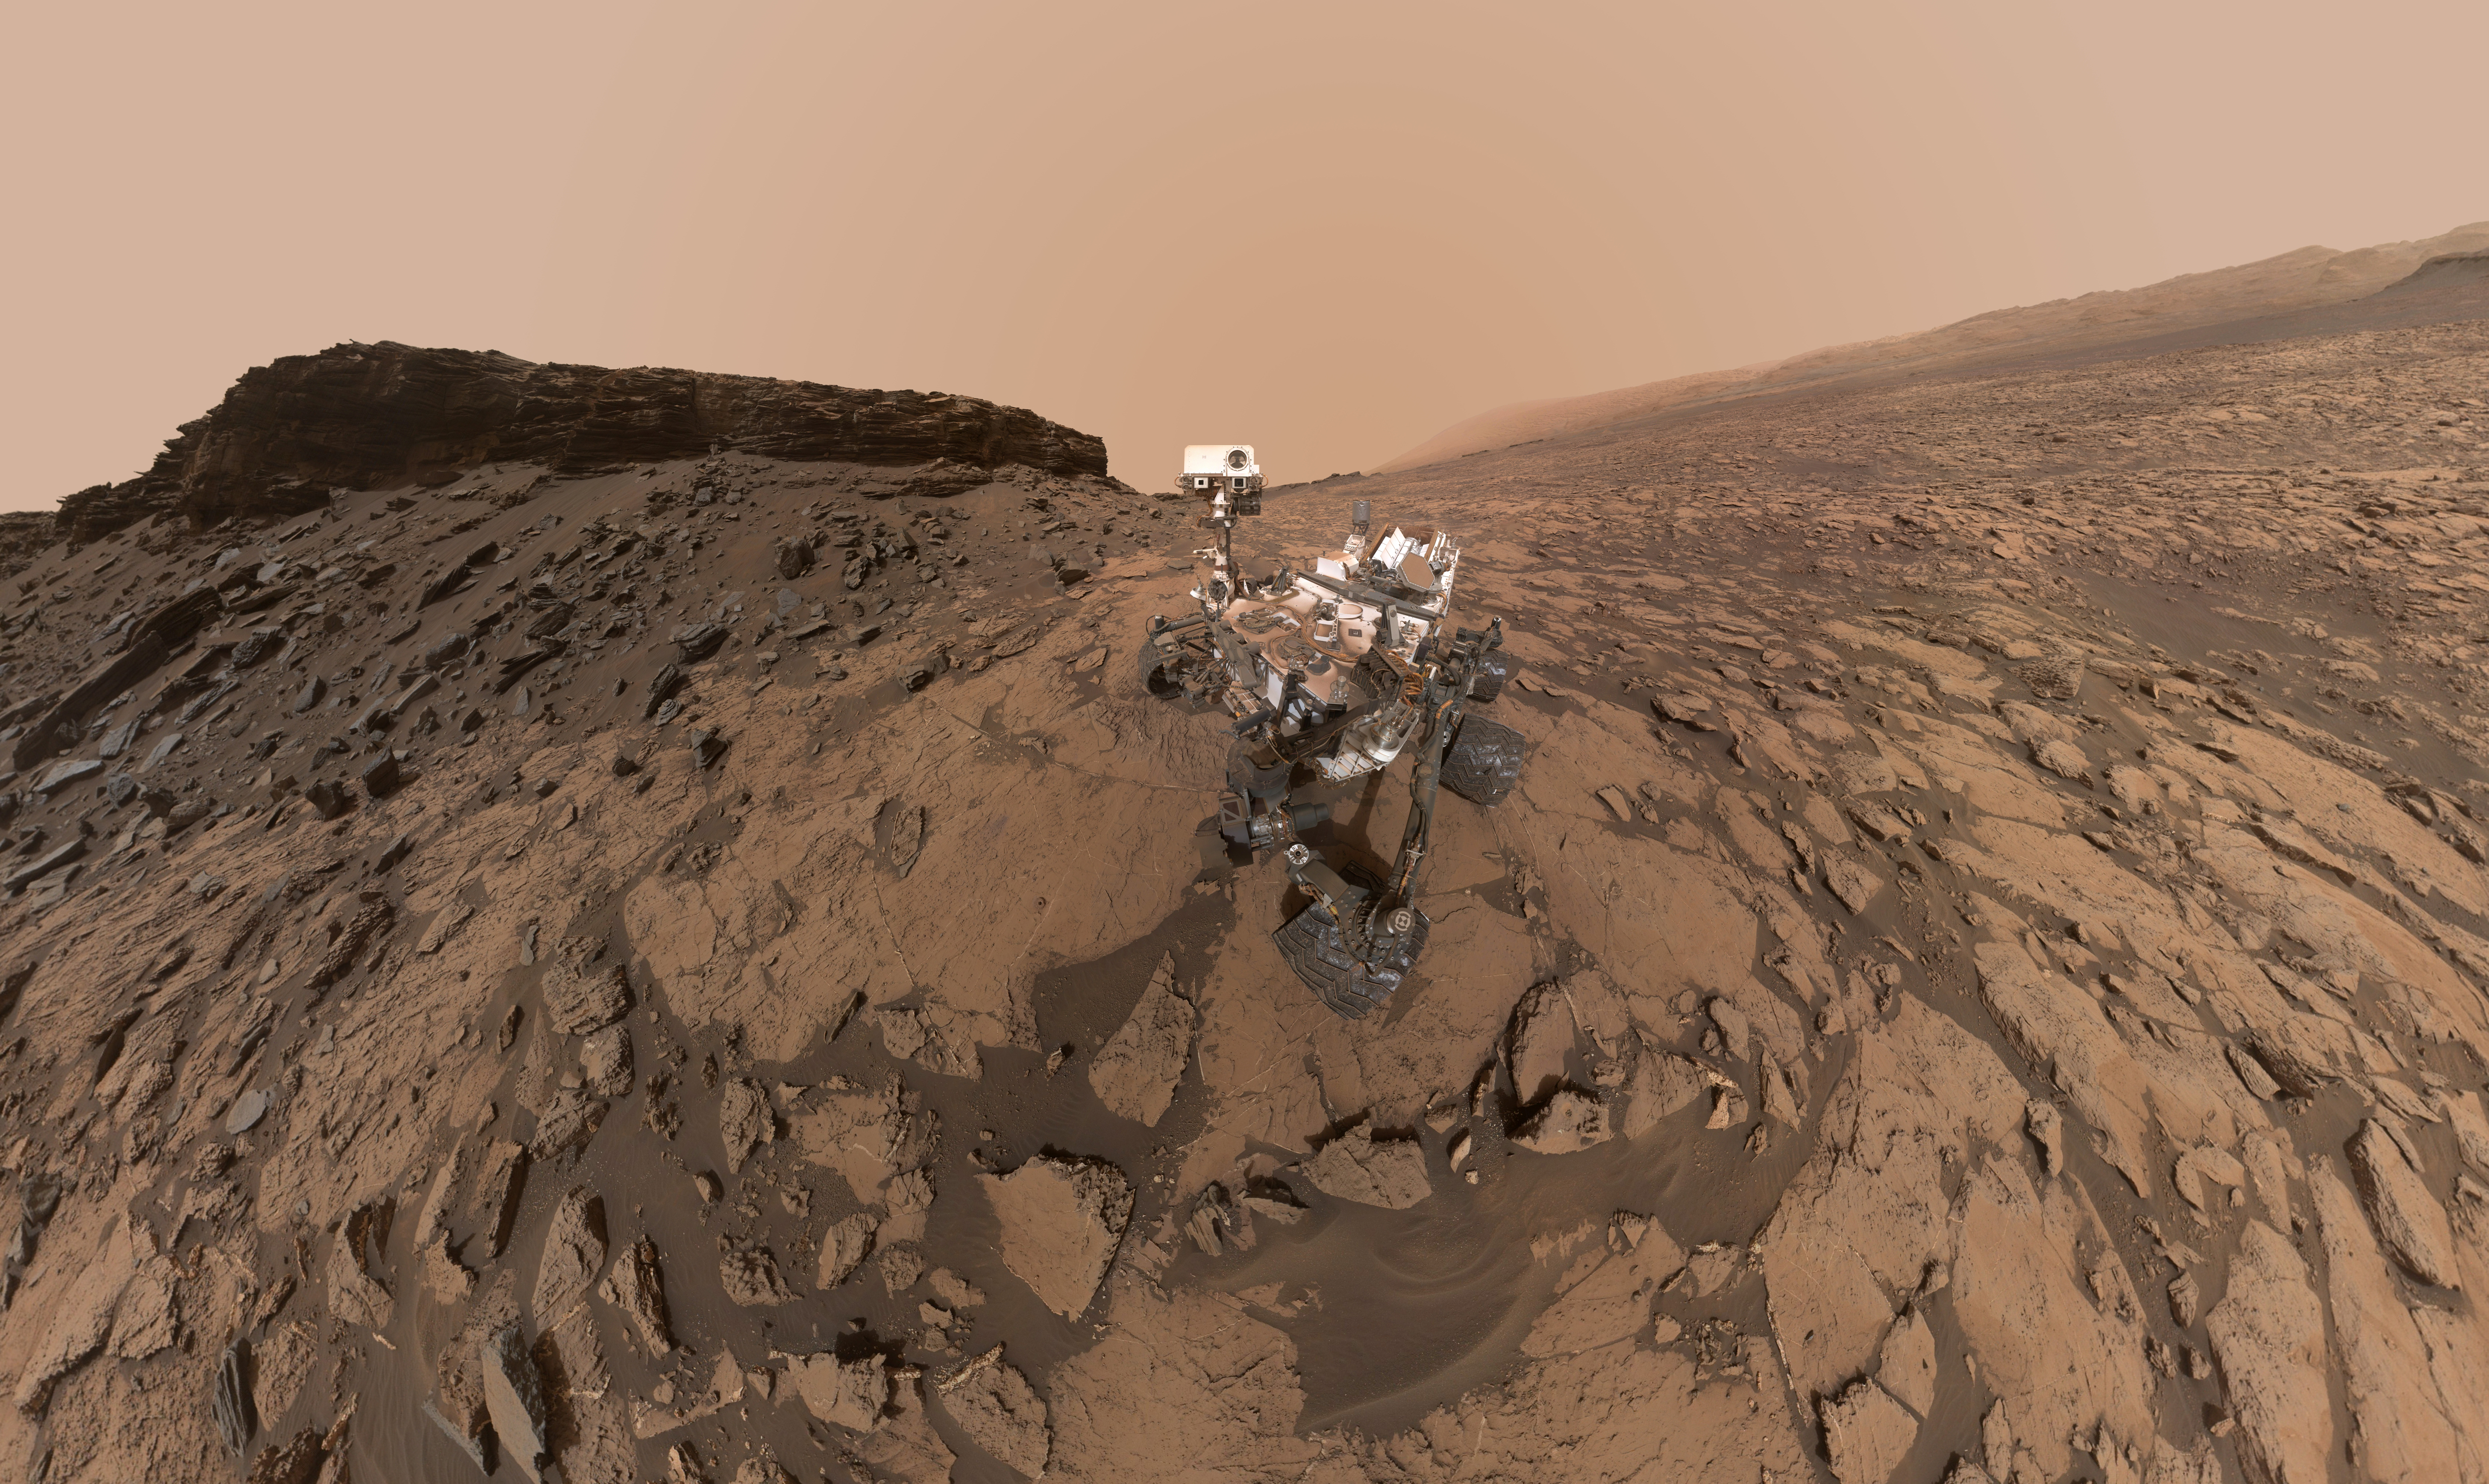
\includegraphics[width=\linewidth]{mars}
			
		{\tiny Curiosity Self-Portrait at 'Murray Buttes',
		\\ Quelle: nasa.gov}}
	\end{minipage}
\end{frame}

\subsection{ESA und Roscosmos - ExoMars}
\begin{frame}{\insertsection: \insertsubsection}
	\begin{minipage}{.45\textwidth}
		
		2016 - 2022: \\
		\textbf{TGO und Schiaparelli} \\
		\note<1>{Schiaparelli
			\begin{itemize}
				\item TGO: Trace Gas Orbiter
				\item Nachweis von Stoffwechselprodukten
				\item Schiaparelli bei Landung (Oktober 2016) zerschellt
			\end{itemize}}
		
		\pause
		
		Ab 2020: \\
		\textbf{ExoMars Rover} \\
			
		\end{minipage} \quad
		\begin{minipage}{.5\textwidth}
			\only<1>{\includegraphics[width=\linewidth]{schiaparelli}
				
				{\tiny ExoMars 2016: Trace Gas Orbiter and Schiaparelli,
					\\ Quelle: esa.int}}
			\only<2>{\includegraphics[width=\linewidth]{exomars}
				
				{\tiny The ExoMars Rover Prototype,
					\\ Quelle: esa.int}}
		\end{minipage}
	\end{frame}

\section{Ferne Zukunft}
\subsection{Erster Unterpunkt}
\begin{frame}{\insertsection: \insertsubsection}
	Goodbye, world!
\end{frame}

\end{document}